\documentclass[12pt,a4paper]{article}
\usepackage[utf8]{inputenc}
\usepackage[T1]{fontenc}
\usepackage{amsmath}
\usepackage{textcomp}

\usepackage{geometry}
\geometry{a4paper,left=25mm,right=25mm, top=2cm, bottom=2cm} 

\usepackage{graphicx} %fuer bilder

\usepackage{verbatim}




 \usepackage{mathptmx}
 \usepackage[scaled=.90]{helvet}
 \usepackage{courier}



\usepackage{listings}
\usepackage{color}
 
\definecolor{dkgreen}{rgb}{0,0.6,0}
\definecolor{gray}{rgb}{0.5,0.5,0.5}
\definecolor{mauve}{rgb}{0.58,0,0.82}

\pagestyle{empty}
\lstset{numbers=left, language=VHDL}
\lstset{showstringspaces=false,
basicstyle=\ttfamily\footnotesize,
breaklines=true,
tabsize=3,
commentstyle=\color{dkgreen},      % comment style
inputencoding={ansinew},
title=\lstname %zeigt titel der datei an
}

\usepackage{pdfpages} % fuer pdfs
\usepackage{hyperref} % fuer url


%keine einrückungen bei absatz
\parindent 0pt

\begin{document}
\title{Übung 04}
\author{Reinhard Penn, Bernhard Selymes, Robert Zeugswetter}
\date{Dezember 2015}

\normalsize


%Beginn des Dokuments

\newcommand{\Uebung}{ScanChainInsertion}
\newcommand{\srcpath}{../../src}
\newcommand{\simpath}{../../sim}
\newcommand{\synpath}{../../syn}

%Angabe
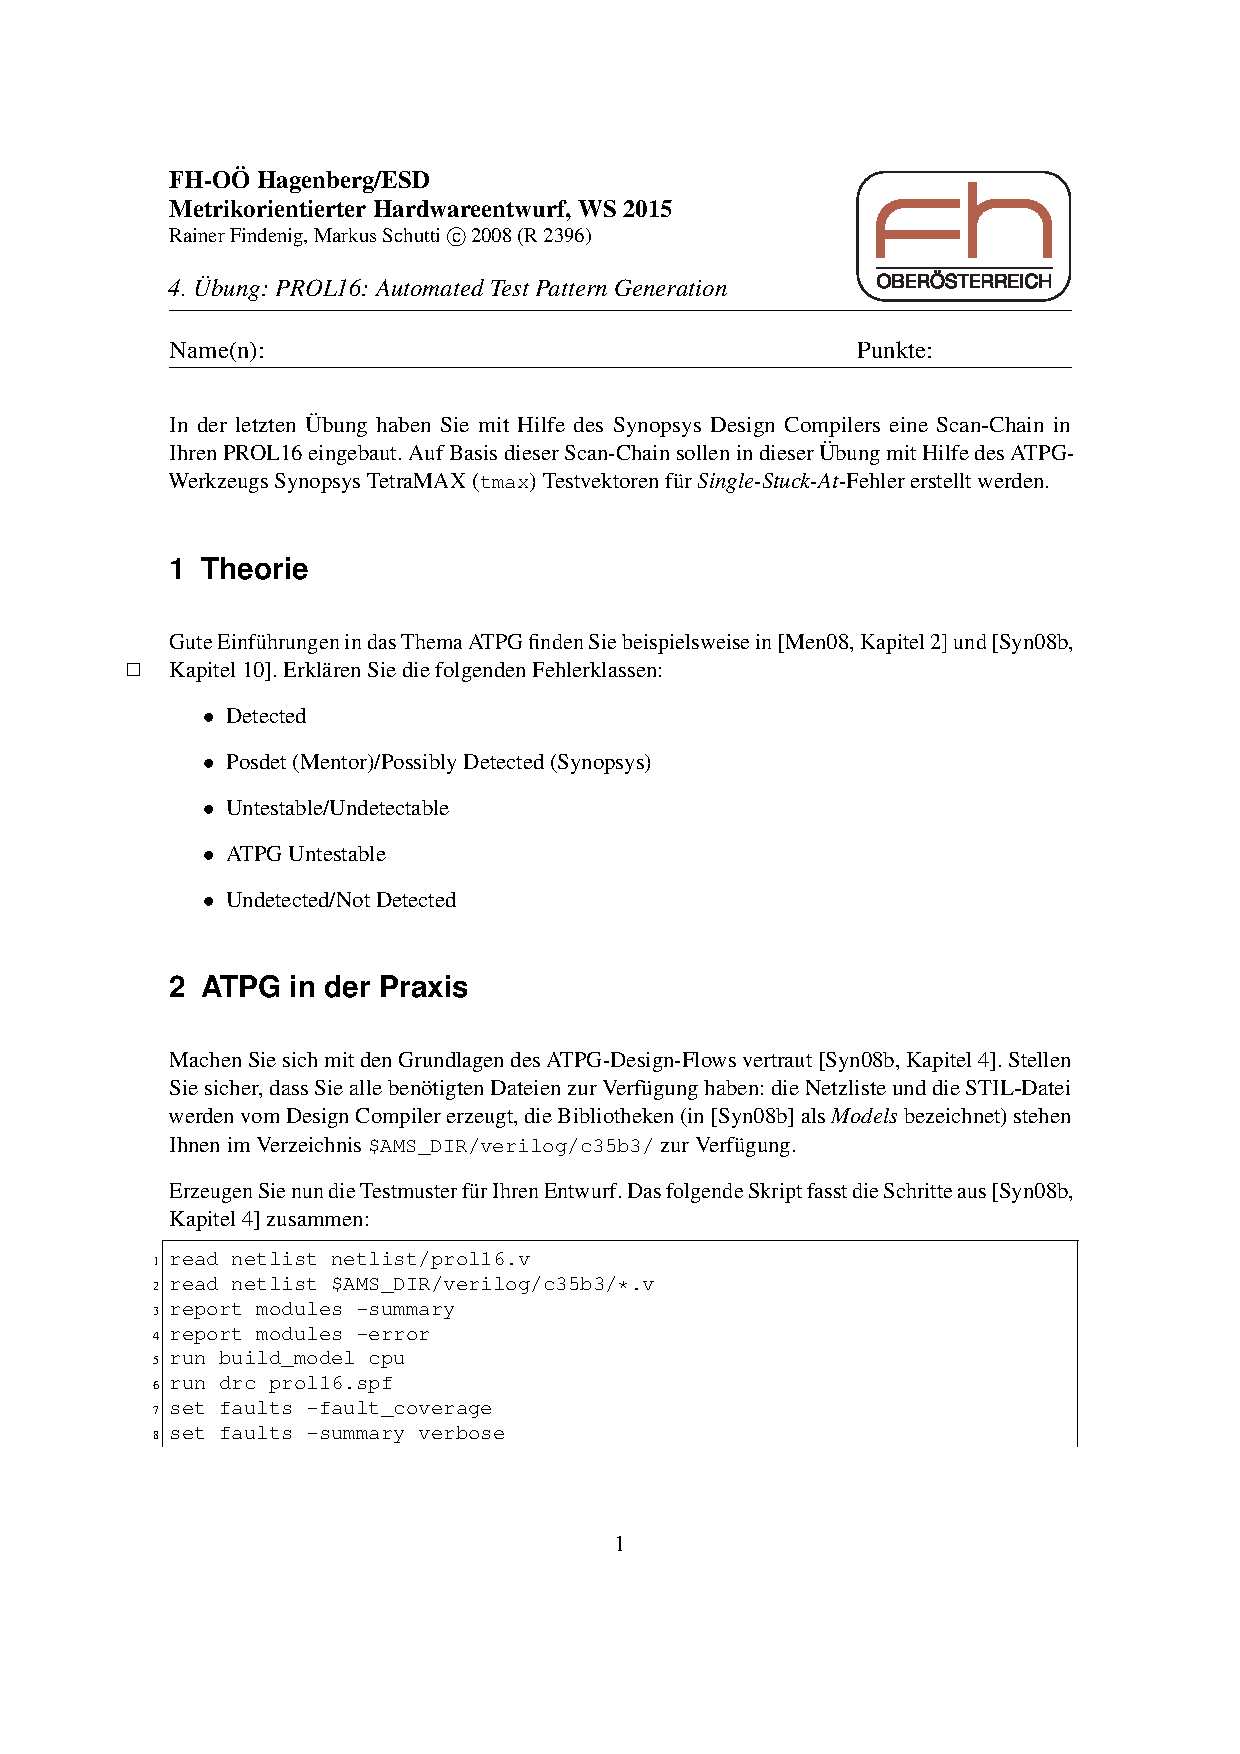
\includepdf[pages=-]{../Angabe.pdf}

\begin{center}
PROL16: Automated Test Pattern Generation\\
Übungsprotokoll zur Übung 4\\
Metrikorientierter Hardwareentwurf\\
Bernhard Selymes, Reinhard Penn, Robert Zeugswetter\\
07.12.2015
\end{center}

\section{Theorie}

Erklärung der Fehlerklassen:

\begin{itemize}

\item Detected\\
Diese Klasse inkludiert alle Faults die vom ATPG erkannt werden. Eine Subkategorie ist Detected by Simulation, hier 
werden Testpatterns generiert und anschließend simuliert um sicherzustellen das mit diesem Testpattern Faults erkannt werden.
Eine andere Subkategorie ist Detected by Implication. Faults dieser Art werden nicht von einem bestimmten Testpattern erkannt.
Sie treten in der Scankette auf, zum Beispiel beim Scanketteneingang oder beim Takt der Scankette.

\item Posdet\\ (Mentor)/Possibly Detected (Synopsys)
Diese Klasse ist in zwei Kategorien unterteilt. Die erste ist ATPG possibly detected. Hier sind alle Faults enthalten für die
nicht bekannt ist ob sie am fehlerhaften Gerät den Wert 0 oder 1 annehmen. Mithilfe einer Analyse ist bewiesen das der Fault
unter derzeitigen ATPG Bedingungen nicht 100% erkannt werden kann. Die Kategorie not analyzed-possibly detected besagt das selbe
mit dem Unterschied das hier das Ergebniss der Analyse ob der Fault unter derzeitigen ATPG Bedingungen 100% erkannt werden kann
inkonklusiv war.

\item Untestable/Undetectable\\
Faults in dieser Klasse können mit keinem Testpattern erkannt werden. Sie beinflussen allerdings auch das Verhalten des
Systems nicht. Eine mögliche Art von Untestable Faults sind die Unused Faults, ein Fault dieser Art kann auftreten wenn 
der Fault an einem offenen Ausgang auftritt. Im Vergleich dazu gibt es auch noch die Klasse Tied, Faults in dieser Klasse
treten auf Pins auf die auf einen bestimmten Wert gesetzt sind. Es kann zum Beispiel ein stuck-at-0 Fault auf einem Pin
der auf 0 hängt nicht erkannt werden. Andere mögliche Arten sind Blocked und Redundant Faults.

\item ATPG Untestable\\
Faults in dieser Klasse können mithilfe von ATPG nicht erkannt werden, aber sie können durch andere Methoden erkannt werden,
zum Beispiel funktionale Tests. Eine Art von Faults in dieser Klasse sind Faults von sequentiellen Elementen die nicht in der
Scankette sind, zum Beispiel Latches.

\item Undetected/Not Detected\\
Faults kommen in diese Klasse wenn die Analyse nicht abgeschlossen oder abgebrochen wurde. Ein möglicher Grund dafür,
ist das erreichen des ATPG Iterationslimit. Die zwei Subkategorien dieser Klasse sind not controlled und not observed.
Not controlled Faults treten auf wenn der ATPG Algorithmus keinen 1 oder 0 erzeugen kann und der Status immer auf X bleibt.
Not observed Faults treten auf wenn die Faults nicht in die Scankette oder an einen Ausgang weitergeleitet werden können.

\end{itemize}

\section{ATPG in der Praxis}

Interpretieren Sie die Ergebnisse, die in die Datei atpg\_results.rep ausgegeben werden! Beschreiben Sie in diesem Zusammenhang auch die beiden Coverage-Werte (siehe [Syn08b, Kapitel 10]).

\section{Simulation der Testmuster}

Erstellen und simulieren Sie nun zwei fehlerhafte Versionen der Netzliste: die erste Version soll einen Single-Stuck-At-Fehler enthalten, der in der Fehlerklasse Detected by Simulation liegt, die zweite einen nicht-detektierbaren Fehler. Dokumentieren Sie die Auswahl und die Vorgehensweise und interpretieren Sie die Ergebnisse.

\end{document}
